\documentclass[11pt]{scrartcl}
\usepackage{graphicx}
\graphicspath{{./}}
\usepackage[sexy]{evan}
\usepackage[normalem]{ulem}
\usepackage{hyperref}
\usepackage{mathtools}
\hypersetup{
    colorlinks=true,
    linkcolor=blue,
    filecolor=magenta,      
    urlcolor=cyan,
    pdfpagemode=FullScreen,
    }

\renewcommand{\dangle}{\measuredangle}

\renewcommand{\baselinestretch}{1.5}

\addtolength{\oddsidemargin}{-0.4in}
\addtolength{\evensidemargin}{-0.4in}
\addtolength{\textwidth}{0.8in}
% \addtolength{\topmargin}{-0.2in}
% \addtolength{\textheight}{1in} 

\newcolumntype{C}{>{\centering\arraybackslash}m{\dimexpr.125\textwidth-2\tabcolsep}}

\setlength{\parindent}{0pt}

\usepackage{pgfplots}
\pgfplotsset{compat=1.15}
\usepackage{mathrsfs}
\usetikzlibrary{arrows}

\title{Coloring}
\author{Pelatihan OSP}
\date{April 2023}

\begin{document}

\maketitle
\begin{soaljawab}
    2023 koin akan diletakkan pada papan berukuran $n \times n$ sedemikian sehingga selisih banyaknya koin pada setiap 2 persegi yang bertetangga adalah 1. Jika 2 persegi disebut bertetangga apabila mereka mempunyai atau berbagi satu sisi yang sama, carilah nilai $n$ terbesar yang mungkin.
    \begin{solusi}
        Perhatikan karena setiap persegi panjang berukuran $2 \times 1$ atau $1 \times 2$ memiliki setidaknya 1 koin, maka $n^2 \le 2023 \times 2$, sehingga $n \le 63$. Akan ditunjukkan bahwa $n=63$ mungkin tercapai.

        Warnai papan 63x63 ini seperti papan catur dengan 1984 kotak hitam dan 1985 kotak putih. Dikarenakan 2023 ganjil, letakkan 1 koin ke setiap 1985 kotak putih yang ada. 38 koin yang tersisa dapat diletakkan pada 16 kotak hitam secara acak dengan setiap kotak tersebut mengandung 2 koin. Hal ini memenuhi soal sehingga $n$ maksimal adalah 63. Terbukti.
    \end{solusi}
\end{soaljawab}

\begin{soaljawab}
    Apakah mungkin untuk berjalan pada taman yang menyerupai papan catur $8 \times 8$ sehingga anda hanya bisa berjalan melewati setiap kotak $1 \times 1$ tepat sekali dengan kotak awal dan kotak akhir perjalanan tersebut berada pada ujung-ujung (corner) yang saling berlawanan? (Anda hanya diperbolehkan berjalan ke kotak yang bertetangga atau tepat bersebelahan dari kotak anda sekarang).
    \begin{solusi}
        Tidak Mungkin. Dengan mewarnai taman tersebut seperti papan catur pada umumnya, dapat disadari setiap kita berdiri di kotak berwarna putih, maka kita hanya bisa berpindah ke kotak berwarna hitam, dan begitu juga sebaliknya. 
        
        Asumsikan tanpa mengurangi keumuman, kotak awal kita berjalan adalah di kotak ujung berwarna putih. Berarti selanjutnya ada 63 kotak tersisa yang bisa dilewati. Perhatikan bahwa langkah pertama kita mau tidak mau pasti ke kotak berwarna hitam. Langkah kedua ke kotak berwarna putih dan seterusnya. Langkah ganjil pasti ke kotak berwarna hitam dan langkah genap pasti ke kotak berwarna putih apapun dan bagaimanapun langkahnya. Karena ada 63 kotak yang harus dilewati menuju kotak akhir dan 63 adalah bilangan ganjil, maka kotak tujuan terakhir yang dilewati haruslah berwarna hitam. Ini kontradiksi dengan fakta bahwa kotak dengan ujung-ujung saling berlawanan harus berwarna sama, yang berarti seharusnya kotak tujuan terakhir berwarna putih.

        Terbukti bahwa perjalanan tersebut tidak mungkin dilakukan.
    \end{solusi}
\end{soaljawab}

\begin{soaljawab}
    Diketahui bahwa delapan persegi panjang berukuran $1 \times 3$ dan satu kotak berukuran $1 \times 1$ menutup papan berukuran $5 \times 5$. Tunjukkan bahwa kotak berukuran $1 \times 1$ tersebut harus berada di tengah papan. (persegi panjang berukuran $1 \times 3$ dan $3 \times 1$ dianggap sama)
    \begin{solusi}
    Warnai 25 kotak satuan pada papan tersebut dengan warna $A,B,C$ seperti berikut.
        \begin{center}
        \begin{tabular}{ |c|c|c|c|c| }
			\hline
			A & B & C & A & B \\
			\hline
			B & C & A & B & C \\
			\hline
			C & A & B & C & A \\
			\hline
			A & B & C & A & B \\
			\hline
			B & C & A & B & C \\
			\hline
		\end{tabular}
        \end{center}
        Ada 8 kotak berwarna $A$, 9 kotak berwarna $B$, dan $8$ kotak berwarna $C$. Perhatikan bahwa setiap persegi panjang $1 \times 3$ menutup masing-masing warna $A,B,C$ satu-satu. Berarti karena ada kelebihan warna $B$, haruslah satu kotak berwarna $B$ ditutupi oleh kotak $1 \times 1$.
        
        Sekarang, akan ditunjukkan bahwa kotak $B$ berukuran $1 \times 1$ tersebut harus berada di tengah. Perhatikan jika papan tersebut dirotasi $90^\circ$ searah jarum jam maka didapat penampakan papannya sebagai berikut.
        \begin{center}
        \begin{tabular}{ |c|c|c|c|c| }
		\hline
		B & A & C & B & A \\
		\hline
		C & B & A & C & B \\
		\hline
		A & C & B & A & C \\
		\hline
		B & A & C & B & A \\
		\hline
		C & B & A & C & B \\
		\hline
	\end{tabular}
        \end{center}
        Perhatikan dari pernyataan serupa seperti sebelumnya, haruslah kotak $1 \times 1$ menutup 1 kotak berwarna $B$ yang ternyata seperti ditunjukkan, sehabis rotasi, masih berada di tengah. Terbukti bahwa kotak $1 \times 1$ harus berada di tengah.
    \end{solusi}
\end{soaljawab}

\begin{soaljawab}
    Dapatkah papan $8\times8$ ditutupi dengan lima belas persegi panjang $1\times4$ dan satu buah persegi $2\times2$ tanpa tumpang tindih?
    \begin{solusi}
        Pertimbangkan pewarnaan papan $8\times8$ berikut:
        \begin{center}
        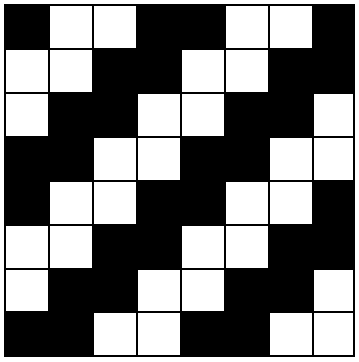
\includegraphics[scale=0.5]{papancaturrev.PNG}
        \end{center}
        Pada pewarnaan papan tersebut, terdapat 32 kotak putih dan 32 kotak hitam. Dengan melihat ilustrasi tersebut, kita dapat melihat setiap persegi panjang $1\times4$ akan menutupi 2 kotak putih dan 2 kotak hitam. Persegi $2\times2$ akan menutupi 1 kotak hitam dan 3 kotak putih atau 3 kotak hitam dan 1 kotak putih. Andaikan pewarnaan pada soal tersebut mungkin Maka 16 potongan bersama-sama harus menutupi entah 31 kotak hitam dan 33 kotak putih atau 33 kotak hitam dan 31 kotak putih, yang merupakan suatu kontradiksi dengan pernyataan sebelumnya.
    \end{solusi}
\end{soaljawab}

\begin{soaljawab}
    Misalkan $m,n > 2$ adalah bilangan bulat. Warnai setiap persegi $1\times1$ dari papan $m\times n$ dengan warna hitam atau putih (tetapi tidak keduanya). Jika dua persegi $1\times1$ yang tepat saling bersebelahan memiliki warna yang berbeda, maka sebut pasangan persegi ini sebagai pasangan "roman". Definisikan $S$ menjadi jumlah pasangan roman di papan $m\times n$. Buktikan bahwa genap atau ganjilnya $S$ hanya tergantung pada persegi $1\times1$ pada pinggiran papan selain 4 persegi $1\times1$ di ujung-ujung sudut papan.
    \begin{solusi}
        Pertama-tama kita membagi persegi $1\times1$ menjadi tiga jenis. Persegi jenis 1 adalah empat persegi $1\times1$ di sudut papan. Persegi jenis 2 adalah persegi $1\times1$ pada pinggiran papan tetapi yang bukan persegi jenis 1. Persegi jenis 3 adalah persegi $1\times1$ yang tersisa. Berikan nilai 1 untuk setiap persegi putih $1\times1$ dan nilai $-1$ untuk setiap persegi hitam $1\times1$. Misalkan persegi jenis 1 masing-masing memiliki nilai $a, b, c, d$. Lalu, misalkan persegi jenis 2 memiliki nilai $x_1, x_2, \dots, x_{2m+2n-8}$ dan persegi jenis 3 memiliki nilai $y_1, y_2, \dots, y_{(m-2)(n-2)}$.
        
        Selanjutnya, untuk setiap pasangan persegi $1\times1$ yang saling bersebelahan, tulislah hasil kali dari nilai-nilai pada dua persegi pada sisi persekutuan mereka (common edge). Definisikan $H$ sebagai hasil kali dari nilai-nilai ini pada semua sisi persekutuan. Untuk setiap persegi jenis 1, terdapat dua persegi tetangga yang berbagi tepi persekutuan dengannya. Oleh karena itu, angka pada persegi jenis 1 muncul dua kali sebagai faktor dalam $H$. Untuk setiap persegi jenis 2, terdapat tiga persegi tetangga yang berbagi tepi persekutuan dengannya. Oleh karena itu, angka pada persegi jenis 2 muncul tiga kali sebagai faktor dalam $H$. Untuk setiap persegi jenis 3, terdapat empat persegi tetangga yang berbagi tepi persekutuan dengannya. Oleh karena itu, angka pada persegi jenis 3 muncul empat kali sebagai faktor dalam $H$. Dengan demikian,

        $$H = (abcd)^2(x_1x_2\dots x_{2m+2n-8})^3(y_1y_2 \dots y_{(m-2)(n-2)})^4 = 1 \cdot (x_1x_2\dots x_{2m+2n-8})^3 \cdot 1$$

        Jika $x_1x_2\dots x_{2m+2n-8} = 1$, maka $H = 1$ dan ada sebanyak genap pasangan berbeda pada papan. Jika $x_1x_2\dots x_{2m+2n-8} = -1$, maka $H = -1$ dan ada sebanyak ganjil pasangan berbeda  pada papan. Oleh karena itu, genap atau ganjil $S$ sepenuhnya ditentukan oleh himpunan kotak tipe 2.
    \end{solusi}
\end{soaljawab}

\begin{soaljawab}
    Terdapat 1004 titik yang berbeda pada sebuah bidang. Hubungkan setiap pasang titik tersebut dan tandai titik tengah dari segmen garis ini dengan warna hitam. Buktikan bahwa terdapat setidaknya 2005 titik hitam pada bidang tersebut dan buktikan ada satu himpunan berisi 1004 titik berbeda yang menghasilkan tepat 2005 titik hitam pada titik tengah dari segmen garis yang menghubungkan pasangan titik-titik tersebut.
    \begin{solusi}
        Dari 1004 titik yang berbeda, kita dapat menggambar $k = {1004 \choose 2}$ segmen garis yang menghubungkan pasangan titik-titik tersebut. Diantara segmen-segmen tersebut, pasti terdapat segmen terpanjang, sebutlah segmen $AB$. Sekarang, titik-titik tengah dari segmen garis yang menghubungkan $A$ dengan 1003 titik lainnya terletak di dalam atau pada lingkaran yang berpusat di $A$ dan berjari-jari $\frac12 AB$. Demikian juga, titik tengah dari segmen garis yang menghubungkan $B$ dengan 1003 titik lainnya terletak di dalam atau pada lingkaran lainnya dengan pusat $B$ dan jari-jari $\frac12 AB$. Kedua lingkaran ini hanya berpotongan (bersinggungan) di titik tengah $AB$. Oleh karena itu, terdapat setidaknya $2 \times 1003 - 1 = 2005$  titik hitam yang dihasilkan oleh segmen garis tersebut ($2 \times 1003$ adalah banyaknya segmen dari $A$ dan $B$ ke titik-titk lainnya dan $-1$ karena persinggungan dua lingkaran tersebut terhitung dua kali). Bagian pertama terbukti.
        
        Untuk membuat konstruksi himpunan 1004 titik yang menghasilkan tepat 2005 titik hitam pada titik tengah dari segmen garis yang menghubungkan pasangan titik tersebut, kita dapat mengambil titik $0, 2, 4, \dots, 2006$ pada sumbu-$x$. Maka titik-titik hitam yang dihasilkan tepat berada pada titik $1, 2, 3, ..., 2005$ pada sumbu-$x$. Bagian kedua terbukti.
    \end{solusi}
\end{soaljawab}

\begin{soaljawab}
    Cari seluruh cara mewarnai semua bilangan positif sedemikian sehingga 
    \begin{enumerate}[(a)]
        \item setiap bilangan positif diberi warna hitam atau putih (tapi tidak keduanya) dan \item jumlah dari dua bilangan dengan warna yang berbeda selalu berwarna hitam dan hasil kali keduanya selalu berwarna putih.
    \end{enumerate}
     
    Tentukan juga warna dari hasil kali dua bilangan yang diwarnai putih.

    \begin{solusi}
        Selain memberi warna yang sama untuk semua bilangan positif, kita juga memiliki pewarnaan berikut yang memenuhi kondisi (1) dan (2). 
        
        Klaim bahwa jika $m$ dan $n$ adalah bilangan putih, maka $mn$ adalah bilangan putih. Untukmembuktikan hal ini, asumsikan $m$ dan $n$ keduanya putih, tetapi $mn$ berwarna hitam. Misalkan bilangan $k$ berwarna hitam. Dari (1), $m+k$ berwarna hitam dan $(m+k)n = mn+kn$ berwarna putih. Di sisi lain, $kn$ berwarna putih dan $mn$ berwarna hitam. Jadi menurut (2), $mn+kn$ juga harus hitam, yang merupakan kontradiksi. Klaim terbukti.
        
        Selanjutnya, misalkan $j$ menjadi bilangan bulat positif putih terkecil (eksistensi $j$ ada dari \textit{well-ordering principle)}. Dari (2) dan klaim, dapat dilihat bahwa setiap $sj$ putih, dengan $s$ adalah sembarang bilangan bulat positif. Akan dibuktikan bahwa setiap bilangan bulat positif $p$ yang bukan kelipatan $j$ berwarna hitam. Dari algoritma Euclid, Tulis $p = qj+r$, dimana $q$ adalah bilangan bulat nonnegatif dan $0 < r < j$. Karena $j$ adalah bilangan bulat positif putih terkecil, maka $r$ harus berwarna hitam. Lalu, perhatikan ketika $q = 0$, maka $p = r$ hitam. Di lain sisi ketika $q \ge 1$, $qj$ berwarna putih dan oleh karena itu menurut (2), $p = qj+r$ hitam.
    \end{solusi}
\end{soaljawab}

\begin{soaljawab}
    Di bidang kartesius, sebuah titik $(x,y)$ disebut sebagai titik letis jika dan
hanya jika $x$ dan $y$ adalah bilangan bulat. Misalkan ada sebuah segi lima konveks $ABCDE$
yang titik-titiknya adalah titik letis dan panjang kelima sisinya adalah bilangan bulat.
Buktikan bahwa keliling segi lima $ABCDE$ adalah bilangan bulat genap.
\begin{solusi}
    Beri warna hitam atau putih pada setiap titik letis $(x,y)$ dari bidang koordinat. Jika $x+y$ genap, maka warnai $(x,y)$ putih. Jika $x+y$ ganjil, maka warnai $(x,y)$ hitam. Perhatikan bahwa $(x,y)$ diberi warna yang berbeda dari empat tetangganya $(x\pm 1,y)$ dan $(x,y\pm 1)$.
    
    Sekarang untuk setiap sisi, dari segi lima $ABCDE$, sebutlah tanpa mengurangi keumuman $AB$,  misalkan $A$ berada di $(x_1, y_1)$ dan $B$ berada di $(x_2, y_2)$. Lalu, misalkan pula $T_{AB}$ adalah titik  yang berada di $(x_1,y_2)$. Kemudian, dari konstruksi secara geometris, $\triangle ABT_{AB}$ adalah sebuah segitiga siku-siku dengan $AB$ sebagai hipotenusa atau sebuah segmen garis (yang dapat dianggap sebagai sebuah \textit{degenerate right triangle}).

     Karena setiap titik letis diberi warna yang berbeda ddari keempat tetangganya, maka sebuah jalur (path) $AT_{AB}BT_{BC}CT_{CD}DT_{DE}ET_{EA}A$ memiliki panjang genap. Untuk bilangan bulat positif $a,b, c$ yang memenuhi $a^2+b^2=c2$, karena $n^2 \equiv n (\mod 2)$ untuk bilangan bulat $n$, maka didapatkan $a+b\equiv c (\mod 2)$. Dengan demikian, keliling $ABCDE$ dan panjang $AT_{AB}BT_{BC}CT_{CD}DT_{DE}ET_{EA}A$ memiliki paritas yang sama. Oleh karena itu, dapat disimpulkan bahwa keliling $ABCDE$ genap.
\end{solusi}
\end{soaljawab}

\begin{soaljawab}
    Sebuah kisi berukuran $5 \times 5$ yang setiap kotaknya berisi lampu-lampu, mengalami kerusakan. Kerusakan ini mengakibatkan setiap memencet sakelar sebuah lampu menyebabkan setiap lampu yang bersebelahan di baris yang sama dan kolom yang sama (beserta lampu itu sendiri) berubah keadaannya, dari nyala menjadi mati, atau dari mati menjadi nyala. Awalnya semua lampu dimatikan. Setelah beberapa kali pemutaran sakelar, tepat satu lampu menyala. Temukan semua posisi yang mungkin dari lampu ini.
    \begin{solusi}
        Beri \textit{label pertama} sebagai berikut untuk masing-masing 25 lampu yang ada pada kisi (dalam ilustrasi berikut 0 dan 1 tidak mesti menotasikan lampu mati dan nyala, tetapi hanya sebagai pelabelan atau pewarnaan saja).
        \begin{center}
        \begin{tabular}{ |c|c|c|c|c| }
		\hline
		1 & 1 & 0 & 1 & 1 \\
		\hline
		0 & 0 & 0 & 0 & 0 \\
		\hline
		1 & 1 & 0 & 1 & 1 \\
		\hline
		0 & 0 & 0 & 0 & 0 \\
		\hline
		1 & 1 & 0 & 1 & 1 \\
		\hline
	\end{tabular}
        \end{center}
        Untuk setiap kombinasi nyala-mati dari lampu dalam kisi, definisikan \textit{nilai pertama}nya sebagai jumlah dari \textit{label pertama} untuk posisi-posisi di mana lampu menyala. Mudah dicek bahwa memencet sakelar selalu menghasilkan kombinasi nyala-mati dari lampu sehingga \textit{nilai pertama}nya mempunyai paritas (genap-ganjil) yang sama seperti \textit{nilai pertama} kombinasi nyala-mati sebelumnya.
        
        Jika diperhatikan, rotasi 90 derajat dari \textit{label pertama} memberikan \textit{label kedua} yang juga membuat paritas dari \textit{nilai kedua} (jumlah dari \textit{label kedua} dari posisi-posisi di mana lampu menyala) tidak berubah saat memencet sakelar.

        \begin{center}
        \begin{tabular}{ |c|c|c|c|c| }
        \hline
        1 & 0 & 1 & 0 & 1 \\
        \hline
        1 & 0 & 1 & 0 & 1 \\
        \hline
        0 & 0 & 0 & 0 & 0 \\
        \hline
        1 & 0 & 1 & 0 & 1 \\
        \hline
        1 & 0 & 1 & 0 & 1 \\
        \hline
        \end{tabular}
        \end{center}
        Karena paritas \textit{nilai pertama} dan \textit{nilai kedua} dari keadaan awal adalah 0, setelah sejumlah proses pemencetan sakelar, paritasnya tetap tidak berubah atau invarian untuk \textit{label pertama} dan \textit{label kedua}. Oleh karena itu, jika hanya satu lampu yang menyala setelah beberapa kali pemencetan sakelar, label posisi itu harus 0 dengan mengacu pada kedua label tersebut. Oleh karena itu, menurut gambar di atas, posisi yang mungkin untuk lampu yang menyala tersebut adalah yang ditandai dengan $*_i$ ($i=0,1,2,3,4$) dalam gambar berikut:
        \begin{center}
        \begin{tabular}{ |c|c|c|c|c| }
        \hline
        ..&  &  &  &  \\
        \hline
        &  $*_2$ &  & $*_1$  &  \\
        \hline
        &  &  $*_0$ &  &  \\
        \hline
        & $*_3$ &  & $*_4 $&  \\
        \hline
        &  &  &  & .. \\
        \hline
        \end{tabular}
        \end{center}
        Sekarang akan didemonstrasikan bahwa semua lima posisi lampu tersebut mungkin:
        Dengan mengganti posisi yang diberi tanda $n$ (urutan penggantian tidak relevan) pada gambar pertama, posisi tengah ($*_0$) adalah satu-satunya posisi yang menyala dan gambar kedua membuat posisi $*_1$ sebagai satu-satunya posisi yang menyala. Posisi $*_i$ yang lain dapat diperoleh dengan memutar gambar kedua dengan suatu putaran.

        \begin{center}
        \begin{tabular}{ |c|c|c|c|c| }
        \hline
        &  &  &  $n$ & $n$ \\
        \hline
        &  & $n$ &  &  \\
        \hline
        &  $n$ &  $n$ &  & $n$ \\
        \hline
        $n$ &  &  & & $n$ \\
        \hline
        $n$ &  & $n$ & $n$ &  \\
        \hline
        \end{tabular}
        \quad
        \begin{tabular}{ |c|c|c|c|c| }
        \hline
        & $n$ &  & $n$ &  \\
        \hline
        $n$ & $n$ &  & $n$ & $n$\\
        \hline
        & $n$ & & & \\
        \hline
        & &$n$ & $n$& $n$ \\
        \hline
        & &  & $n$ & \\
        \hline
        \end{tabular}
        \end{center}
    \end{solusi}
\end{soaljawab}

\begin{soaljawab}
    % nordic 2020
    Ultrawati memiliki $2n + 1$ kartu dengan sebuah angka ditulis pada setiap kartu. Pada salah satu kartu terdapat angka 0, dan di antara sisa kartu yang ada, bilangan bulat $k = 1, \dots, n$ muncul masing-masing dua kali. Ultrawati ingin meletakkan kartu-kartu tersebut dalam satu baris sedemikian sehingga kartu 0 berada di tengah, dan untuk setiap $k = 1, ..., n$, kedua kartu dengan angka $k$ memiliki jarak $k$ (yang berarti ada tepat $k - 1$ kartu di antara mereka). Untuk nilai $n$ berapa saja, dengan $1 \le n \le 10$, hal ini dimungkinkan?

    \begin{solusi}
        Pertimbangkan pewarnaan $2n+1$ ruangan yang nantinya akan diisi dengan kartu-kartu dengan setiap ruangan tersebut diwarnai hitam dan putih secara bergantian dan setiap ruang tersebut diberi nomor $1,2,\dots,2n+1$ dari kiri ke kanan. Tanpa mengurangi keumuman, kita dapat mengasumsikan bahwa dua ruangan di ujung baris, ruangan pertama dan terakhir, keduanya berwarna hitam. 
        \begin{center}
            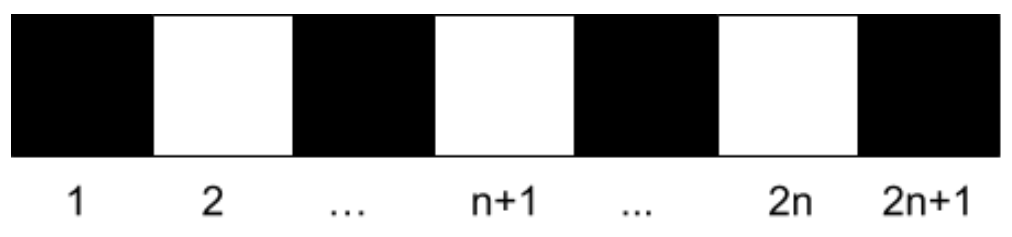
\includegraphics[scale=0.3]{nordic}
        \end{center}
        Karena pola tersebut bergantian, dari $2n+1$ ruang, $n+1$ akan berwarna hitam dan $n$ ruang akan berwarna putih. 
        \vspace{10pt}
        Perhatikan bahwa ruang tengah selalu bernomor $n+1$. Karena ruang pertama berwarna hitam, semua ruang dengan nomor ganjil berwarna hitam, sedangkan ruang dengan nomor genap berwarna putih. 
        \vspace{10pt}
        Jika $n$ genap, maka $n+1$ bernilai ganjil sehingga ruang tengah akan berwarna hitam. Karena ada $n+1$ ruang berwarna hitam, maka ada sebanyak ganjil ruang hitam. Dari sini jelas bahwa di sebelah kanan dan kiri ruang tengah, masing-masing ada $\frac{n}{2}$ ruang hitam dan ruang putih.
        \vspace{10pt}
        Jika $n$ ganjil, ruang tengah akan berwarna putih. Berarti ada $n-1$ ruang putih sisanya selain ruang tengah dan $n+1$ ruang hitam dimana ruang-ruang tersebut terdistribusi secara merata di kanan dan kiri ruang tengah.
        \vspace{10pt}
        Sekarang perhatikan saat sepasang kartu ditempatkan di ruang-ruang tersebut. Misalkan sepasang kartu tersebut memiliki angka $k$. Asumsikan kartu tersebut dapat ditempatkan sesuai aturan di soal, maka salah satu kartu menempati ruang bernomor $m$ dan kartu lainnya menempati ruang bernomor $m+k$. Jika $k$ genap, maka dua ruang tersebut akan memiliki paritas (ganjil-genap) yang sama. Namun, jika $k$ ganjil, maka dua ruang tersebut akan berbeda paritasnya yang sekaligus berbeda warnanya.
        \vspace{10pt}
        Akan ditunjukkan bahwa skenario penyusunan kartu akan gagal saat $n \equiv 1 \mod 4$. Dalam skenario ini, jelas bahwa $n$ ganjil, sehingga kartu bernomor bukan 0 akan menempati $n-1$ ruang putih dan $n+1$ ruang hitam. Akan tetapi, ada sebanyak ganjil pasangan kartu yang bernomor ganjil. Jika diobservasi ruang putih yang harus ditempati oleh kartu, kita bisa melihat bahwa ada sebanyak genap ruang putih di keadaan awal. Namun, karena untuk setiap pasang kartu yang bernomor ganjil harus menempati tepat satu ruang putih, maka akan ada sebanyak ganjil ruang putih tersisa untuk pasangan kartu bernomor genap. Hal ini tidaklah mungkin, karena sepasang kartu bernomor genap selalu menempati sebanyak genap ruang putih (0 atau 2 ruang), sehingga banyaknya ruang putih ditempati oleh pasangan kartu genap akan selalu genap dan tidak pernah ganjil. Dari sini jelas bahwa $n=1,5,9$ tidak mungkin.
        \vspace{10pt}
        Sekarang, dengan cara yang mirip dengan sebelumnya, akan ditunjukkan bahwa skenario penyusunan kartu juga akan gagal saat $n \equiv 2 \mod 4$. Pada skenario ini, jelas bahwa $n$ genap, sehingga kartu bernomor bukan 0 harus menempati $n$ ruang putih dan $n$ ruang hitam. Karena $n=4k+2$, untuk suatu $k$ cacah, maka akan selalu ada sebanyak ganjil pasangan kartu genap dan sebanyak ganjil kartu ganjil. Selanjutnya, ada sebanyak genap ruang putih dan sebanyak ganjil pasangan kartu ganjil yang harus menempati sebanyak ganjil ruang putih. Hal ini berarti tersisa sebanyak ganjil ruang putih untuk pasangan kartu genap. Tentu saja skenario ini mustahil terjadi dari fakta-fakta sebelumnya, sehingga dapat disimpulkan kasus $n=2,6,10$ otomatis gagal.

        Akan dikonstruksi konfigurasi kasus $n=3,4,7,8$ yang memenuhi:
        \begin{itemize}
            \item Untuk $n=3$ konfigurasi yang memenuhi adalah 2 3 2 0 3 1 1
            \item Untuk $n=4$ konfigurasi yang memenuhi adalah 2 4 2 3 0 4 3 1 1
            \item Untuk $n=7$ konfigurasi yang memenuhi adalah 3 7 2 3 2 6 4 0 7 5 4 6 1 1 5
            \item Untuk $n=8$ konfigurasi yang memenuhi adalah 5 8 2 3 2 5 3 7 0 8 6 4 1 1 7 4 6
        \end{itemize}
        Oleh karena itu, kesimpulannya hanyalah $n=3,4,7,8$ yang membuat penyusunan kartu tersebut dimungkinkan.
    \end{solusi}
\end{soaljawab}
\end{document}
